% !TEX TS-program = lualatex
\documentclass[10pt]{article}
\usepackage[a4paper,margin=16mm]{geometry}
\usepackage{amsmath,amssymb}
\usepackage{luatexja}
\usepackage{tikz}
\usetikzlibrary{arrows.meta}
\pagestyle{empty}

\begin{document}
\begin{center}
  {\Large 2022年 東京大学 理系数学 第5問}\par
  \vspace{1mm}
  {\small 回転面上の点と線分の中点がつくる立体}
\end{center}

点 $A(0,0,2)$ と点 $B(1,0,1)$ を結ぶ線分 $AB$ を $z$ 軸のまわりに
回転して得られる曲面を $S$ とする。$S$ 上の点 $P$ と $xy$ 平面上の点
$Q$ が $PQ=2$ を満たして動くとき、線分 $PQ$ の中点 $M$ の通過範囲を
$K$ とする。以下、$K$ の体積を求める。

\medskip
\noindent\textbf{1. 回転面と点 $P$ の表示}

線分 $AB$ 上では、$z=p$ とおくと原点からの水平距離は $2-p$ である。
したがって曲面 $S$ は
\[
  1\le p\le2,\qquad x^2+y^2=(2-p)^2
\]
と表される。回転対称性より、$P$ を含む鉛直半平面を改めて $xz$ 平面と
すれば
\[
  P=(2-p,0,p)\qquad(1\le p\le2)
\]
と固定して考えてよい。

\begin{center}
% 作図ツールで〈図1〉をここに挿入する
%% tex64-figure v2 h=70d2f171 /3sidiI6MSwi/3VuaXQiOiJt/20iLCJ3aWR0/WgBUDAwLCJoZedpZ2gBkADCZ3Jp/2QiOnsic2l6/2UiOjUsInNu/2FwIjpmYWxz+2V9ANB0eWxlc/8iOltdLCJvYm9qZWN0AMF7IgNB/yIxMHVzdXZ07gXgdHlwA9AicGHsBkADQWFyBfB7Inh8BRAGMHkiOjMwBMGfZWdtZW4EFAMkbNdpbmUEAW8C+zgw+319ByBjbG9zZfAGoAjiCNQCgXByb3CqBGB7A+JXDbFQDQEsfyJhcnJvd1MH89kiBXAA8kVuCtFTdPdlYWwJ8H19fSx+DAUxc2g5YXIMD/AMDwwPDA8C8jMxLjnfOTc4NjIDYjE1wAx/DH8Mfwx/DH8MeDJ1D2h3NmMMfwx/DH8Mf/4C8jc2LjY0MzG7NzMMczguNA1AM4EyDO8M7wzvDO8M7wzoM58xY3RpeQzvDO83+AzvDO8ZYjcuNzU49zU0OQNiNTEuMsE3AAAZ3wzvDO4KmTQwDzVteW8KnwqfCp8Kn/4C8jYyLjI0MTSDNTgKnwqfCp8KnwqTNd94Yjg3NQqXZWyvbGlwcweRYwkQZWlyCtsHYDksMDgzC0DVcgFgMQlHcgHgNC4/MzIwNTE0CC8IL34IJzZvb3Z2MhLP/hLINDMuODc5Mvk3SIAGYDYwLjY3DzU2NTITrxOvE6EeQA84NjExKzMuoBM/Cw/8Cw8LBjc3cXZraq4LB25vZAbxYR2mMr8uNjgwNjIK0zi9MAfQOTcwOArQbLdhdGUCACJ6AuFuh2NobxXwFoUINwaoOJ95ODRkMQavBqUzfzAuMDY5OTM45L4SYDIxNzQ2Bqh4+AavBq8GoWFvd2xl+BNyBq8YMjguMDcy/AAgK3MyLjE0ODbFNw1ZQQavBq8GoWJoTzZrZ3cGrw1WNRQARzY2MEIgJ0wGpUIGr3wGrwahY21qeW0UDzoNVzAlkDEyMTVjNkAtNzDgNjcGqFAGrwavfgahZDF5a2hpBq92BqU2OStgNDY0DVO9MgDQNjM2MgapUfgGrwavBqFmdjVodPkzBq8GpjUuMzU01zEyNw1VMAeQODHiBqhTBq8GrwahZ2p65282ZAavLsY2LjfvMTMwOVQTNDYuPzIyNTU5NQaoPaH8Bq8GrzFodGkwbbQoHwamOCCAMTYGpTF/NS4yNjE5MUBR8AalYcEGrwavMWkyMtNpdCgfIWc3FAAxOe04IWMyNhQAMzE5Mhq5TwavBqpdfQ==
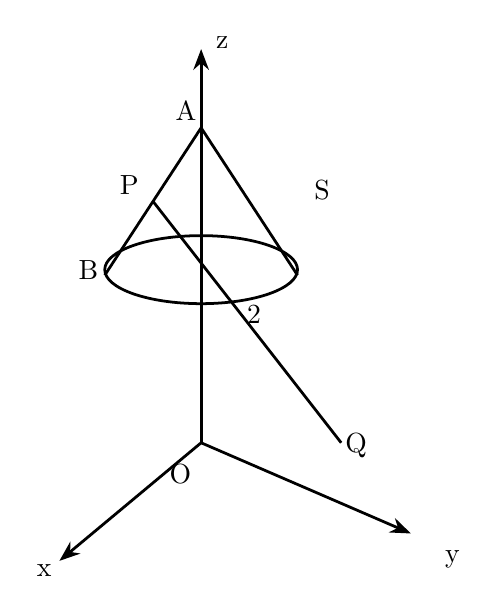
\begin{tikzpicture}[x=1mm, y=1mm]
  \draw[line width=1pt, -{Stealth}] (50,30) -- (50,80);
  \draw[line width=1pt, -{Stealth}] (50,30) -- (31.998,15);
  \draw[line width=1pt, -{Stealth}] (50,30) -- (76.643,18.479);
  \draw[line width=1pt] (50,70) -- (37.759,51.278);
  \draw[line width=1pt] (50,70) -- (62.241,51.278);
  \draw[line width=1pt] (50,51.986) ellipse [x radius=12.241, y radius=4.321];
  \draw[line width=1pt] (43.879,60.676) -- (67.786,30);
  \node at (52.681,80.79) {z};
  \node at (30.07,13.822) {x};
  \node at (48.072,72.149) {A};
  \node at (35.687,51.986) {B};
  \node at (40.871,62.788) {P};
  \node at (69.675,29.664) {Q};
  \node at (65.354,62.067) {S};
  \node at (56.713,46.226) {2};
  \node at (81.916,15.262) {y};
  \node at (47.352,26.063) {O};
\end{tikzpicture}

{\small 〈図1〉曲面 $S$、線分 $AB$、および $PQ=2$}
\end{center}

$P$ の $xy$ 平面への正射影を $R=(2-p,0,0)$ とする。$Q$ は $xy$ 平面上に
あり、直角三角形 $PRQ$ について $PR=p$, $PQ=2$ だから
\[
  RQ^2+p^2=4,\qquad RQ=\sqrt{4-p^2}.
\]
よって、$P$ を固定したとき $Q$ は、中心 $R$、半径 $\sqrt{4-p^2}$ の円を
$xy$ 平面上に描く。

\medskip
\noindent\textbf{2. 高さ $z=m$ における $K$ の断面}

$M$ は $PQ$ の中点なので、その $z$ 座標を $m$ とおけば
\[
  m=\frac p2,\qquad \frac12\le m\le1.
\]
固定した $P$ に対し、$M$ の水平成分は $Q$ の水平成分を $1/2$ に縮小した
ものだから、$M$ は高さ $z=m$ の平面上で、中心が $P$ の水平成分と一致し、
半径
\[
  \frac12\sqrt{4-p^2}=\sqrt{1-m^2}
\]
の円を描く。

さらに $P$ 自身を $z$ 軸のまわりに回転させると、この円の中心は半径
\[
  2-p=2(1-m)
\]
の円周上を動く。したがって $K$ の高さ $z=m$ における断面は、外半径
$2(1-m)+\sqrt{1-m^2}$、内半径
$\lvert2(1-m)-\sqrt{1-m^2}\rvert$ の環状領域である。
ゆえに断面積 $S(m)$ は
\begin{align*}
 S(m)
 &=\pi\{2(1-m)+\sqrt{1-m^2}\}^{2}
   -\pi\{2(1-m)-\sqrt{1-m^2}\}^{2}\\
 &=8\pi(1-m)\sqrt{1-m^2}.
\end{align*}

\medskip
\noindent\textbf{3. 断面積の積分}

以上より
\begin{align*}
 V
 &=\int_{1/2}^{1}S(m)\,dm\\
 &=8\pi\left(
      \int_{1/2}^{1}\sqrt{1-m^2}\,dm
      -\int_{1/2}^{1}m\sqrt{1-m^2}\,dm
    \right).
\end{align*}
ここで
\[
 \int_{1/2}^{1}\sqrt{1-m^2}\,dm
   =\frac{\pi}{6}-\frac{\sqrt3}{8},\qquad
 \int_{1/2}^{1}m\sqrt{1-m^2}\,dm
   =\frac{\sqrt3}{8}.
\]
したがって、求める体積は
\[
 \boxed{V=8\pi\left(\frac{\pi}{6}-\frac{\sqrt3}{4}\right)
 =\frac{4}{3}\pi^2-2\sqrt3\,\pi}.
\]

\end{document}
